\newpage
\section{Classification Models (Trainable Vectorization and Emebddings)}
La clasificación de los modelos en conjunto con su vectorización y los \textit{embeddings} inicia con la búsqueda de los mejores hiper parámetros mediante una búsqueda de grilla modificada. En un principio, la búsqueda de grilla debería variar una serie de hiper parámetros con el fin de encontrar los que producen un mejor modelo. Sin embargo, variar todos los parámetros dentro de una misma búsqueda implica entrenar y evaluar múltiples modelos, lo cual requiere una gran cantidad de tiempo y recursos computacionales. Con el fin de disminuir el tiempo dedicado a la búsqueda de los hiper parámetros se realiza una búsqueda de cada valor de forma independiente. Esta aproximación se ve favorecida por el conocimiento previo del problema y de algunos valores obtenidos en etapas previas del desarrollo del problema. \\

\subsection{Búsqueda de Hiper Parámetros}

La búsqueda de los hiper parámetros se hace variando los valores correspondientes a la dimensionalidad del embedding, la longitud de las sentencias y el tamaño del vocabulario. El orden en el cual se realiza esta búsqueda está determinado por el hecho de que se conocen datos de la longitud de las sentencias y del tamaño del vocabulario. En este sentido, el primer parámetro a buscar corresponde a la dimensionalidad del embedding, seguido de la longitud de las sentencias y finalizando con el tamaño del vocabulario. Vale la pena mencionar que otras condiciones relacionadas a los modelos, como lo son instancias de regularización y variaciones en la vectorización, van a ser evaluadas posteriormente. \\

Para realizar la búsqueda de los parámetros se utiliza un modelo, descrito en la tabla \ref{tab:deep_em_hyper_params}, de una red neuronal completamente conectada (FCN, \textit{Fully Connected Network}). La primera capa de la red corresponde a la de vectorización de texto que oficia como entrada al modelo, recibiendo las sentencias a clasificar. La salida de la capa de vectorización corresponde a una secuencia con una cantidad dada de tokens denotados por \textit{seq\_len}. Una vez se ha vectorizado el texto, este entra a la capa de embedding cuya dimensionalidad va a estar dada por \textit{seq\_len} y \textit{embedding\_dim} que representa la dimensionalidad del embedding. La capa de embedding presenta una salida de dos dimensiones que debe ser ajustada para alimentar las capas densas de la red neuronal. Para dicho ajuste se usa una capa que calcula el promedio global de cada embedding, convirtiendo así la salida de dos dimensiones en un vector con \textit{embedding\_dim} dimensiones. La capa densa de la red contienen un número de neuronas que se calcula con el promedio entre \textit{embedding\_dim} y \textit{output\_dim}, que corresponde al número de clases que serán clasificadas. Finalmente, la última capa contiene \textit{output\_dim} neuronas con el fin de realizar la clasificación correspondiente. \\

\begin{table}[H]
    \centering
    \begin{tabular}{|l|l|}
        \hline
        \textbf{Tipo de Capa} & \textbf{Características} \\ \hline
        Vectorización de Texto & Denotada por \textit{seq\_len} \\ \hline
        Embedding & Denotada por \textit{seq\_len} y \textit{embedding\_dim} \\ \hline
        Promedio Global de 1D & Convierte los valores a una dimensión \\ \hline
        Densa & Neuronas: promedio entre \textit{embedding\_dim} y \textit{output\_dim} \\ \hline
        Densa & Neuronas: dado por \textit{output\_dim} \\ \hline
    \end{tabular}
    \caption{Definición del modelo para la evaluación y selección de hiper parámetros.}
    \label{tab:deep_em_hyper_params}
\end{table}

La primera etapa de la búsqueda de hiper parámetros se dedicó a fijar la dimensionalidad del embedding. Las posibles dimensiones consideradas fueron de 5, 10, 15, 20, 25, 50, 100 y 150. Las figuras \ref{fig:em_embedding_simpsons} y \ref{fig:em_embedding_friends} presentan respectivamente los resultados para los dos conjuntos de datos: el de \textit{Los Simpsons} y \textit{Friends}. Se puede identificar que los mejores resultados se obtienen con una dimensión de 150 para los dos conjuntos de datos. Vale la pena notar que los modelos para el conjunto de datos de \textit{Friends} demuestran aprendizaje, pero con bajos niveles de recall.  \\

\begin{figure}[H]
    \centering
    \begin{subfigure}[b]{0.45\textwidth}
        \centering
        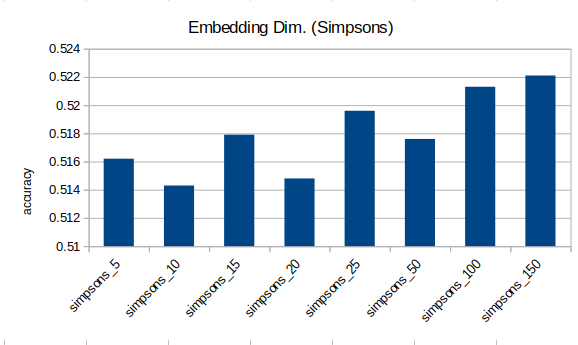
\includegraphics[width=\textwidth]{doc/images/em_models/embedding_dim_simpsons.png}
        \caption{Métricas de evaluación para diferentes dimensiones del embedding en el conjunto de datos de \textit{Los Simpsons}.}
        \label{fig:em_embedding_simpsons}
    \end{subfigure}
    \hfill
    \begin{subfigure}[b]{0.45\textwidth}
        \centering
        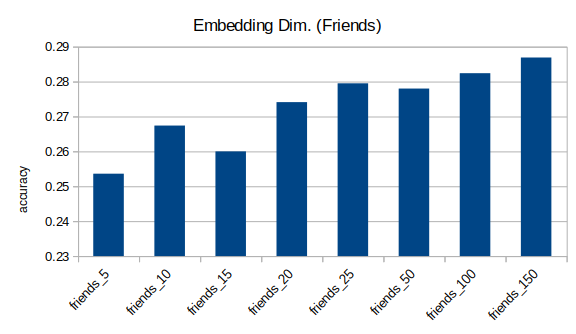
\includegraphics[width=\textwidth]{doc/images/em_models/embedding_dim_friends.png}
        \caption{Métricas de evaluación para diferentes dimensiones del embedding en el conjunto de datos de \textit{Friends}.}
        \label{fig:em_embedding_friends}
    \end{subfigure}
    \caption{Métricas de evaluación para la búsqueda de la mejor dimensión del embedding.}
    \label{fig:em_embedding}
\end{figure}

Una vez se ha definido la mejor dimensión para el embedding, se procede a evaluar distintas longitudes de las secuencias. Siguiendo un procedimiento similar al usado para las dimensiones del embedding, se define una serie de posibles longitudes para las secuencias. En este caso las longitudes consideradas fueron: 5, 10, 15, 20, 25, 50 y 100. Los resultados de esta búsqueda se presentan en la figura \ref{fig:em_seq_len}. A partir de los resultados se puede establecer que el mejor modelo corresponde a una longitud de secuencia de 15 para el conjunto de datos de \textit{Los Simpsons} y 20 para el conjunto de datos de \textit{Friends}.

\begin{figure}[H]
    \centering
    \begin{subfigure}[b]{0.45\textwidth}
        \centering
        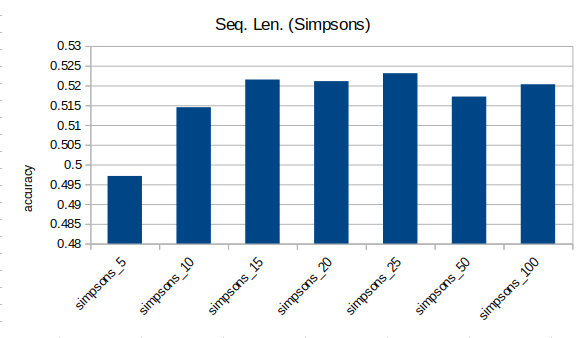
\includegraphics[width=\textwidth]{doc/images/em_models/seq_len_simpsons.png}
        \caption{Métricas de evaluación para diferentes longitudes de las secuencias en el conjunto de datos de \textit{Los Simpsons}.}
        \label{fig:em_seq_len_simpsons}
    \end{subfigure}
    \hfill
    \begin{subfigure}[b]{0.45\textwidth}
        \centering
        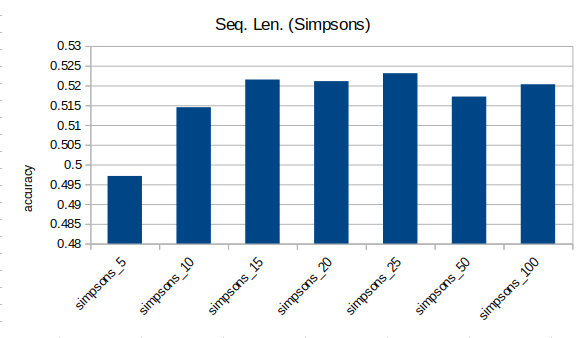
\includegraphics[width=\textwidth]{doc/images/em_models/seq_len_simpsons.png}
        \caption{Métricas de evaluación para diferentes longitudes de las secuencias en el conjunto de datos de \textit{Friends}.}
        \label{fig:em_seq_len_friends}
    \end{subfigure}
    \caption{Métricas de evaluación para la búsqueda de la mejor longitud de secuencia.}
    \label{fig:em_seq_len}
\end{figure}

El último hiper parámetro que hace parte de la búsqueda corresponde al tamaño del vocabulario. Para esta búsqueda se consideran tamaños de vocabulario de 1000, 2500, 5000, 10000 y 15000. Los resultados de la búsqueda del mejor tamaño de vocabulario se presentan en la figura \ref{fig:em_vocabulary_size}. De los resultados presentados se puede establecer que el mejor tamaño de vocabulario es de 10000 para el conjunto de datos de \textit{Los Simpsons} y de 15000 para el conjunto de datos de \textit{Friends}.

\begin{figure}[H]
    \centering
    \begin{subfigure}[b]{0.45\textwidth}
        \centering
        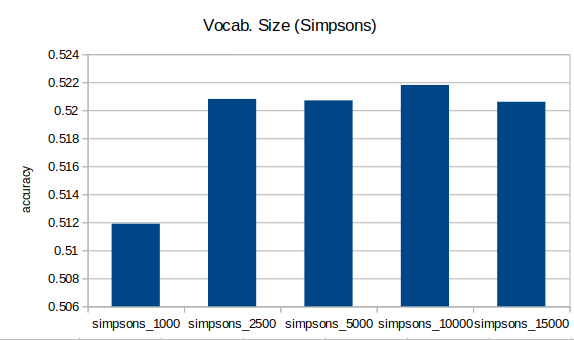
\includegraphics[width=\textwidth]{doc/images/em_models/vocab_size_simpsons.png}
        \caption{Métricas de evaluación para diferentes tamaños de vocabulario en el conjunto de datos de \textit{Los Simpsons}.}
        \label{fig:em_vocabulary_size_simpsons}
    \end{subfigure}
    \hfill
    \begin{subfigure}[b]{0.45\textwidth}
        \centering
        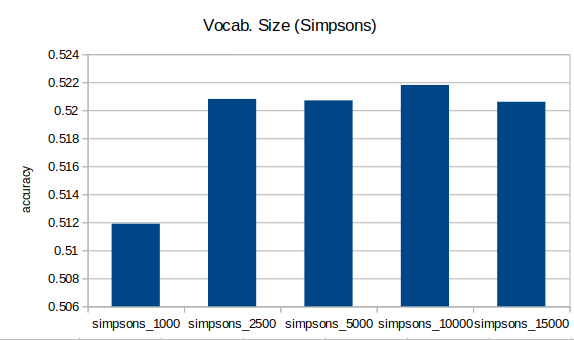
\includegraphics[width=\textwidth]{doc/images/em_models/vocab_size_simpsons.png}
        \caption{Métricas de evaluación para diferentes tamaños de vocabulario en el conjunto de datos de \textit{Friends}.}
        \label{fig:em_vocabulary_size_friends}
    \end{subfigure}
    \caption{Métricas de evaluación para la búsqueda del mejor tamaño del vocabulario.}
    \label{fig:em_vocabulary_size}
\end{figure}

A partir de los resultados obtenidos en las tres búsquedas presentadas previamente se pueden establecer los hiper parámetros que serán usados en la etapa de selección de modelos. La tabla \ref{tab:em_hyper_params} resume estos hiper parámetros para cada conjunto de datos. Para la etapa de selección de modelos se procede a evaluar diferentes arquitecturas profundas para la clasificación de las sentencias en los dos conjuntos de datos.

\begin{table}[H]
    \centering
    \begin{tabular}{|c|c|c|c|}
        \hline
        \textbf{Conjunto } & \textbf{Dimensión de} & \textbf{Longitud de} & \textbf{Tamaño del}  \\
        \textbf{de datos} & \textbf{embedding} & \textbf{secuencia} & \textbf{vocabulario} \\ \hline
        Los Simpsons & 150 & 15 & 10000 \\ \hline
        Friends & 150 & 20 & 15000 \\ \hline
    \end{tabular}
    \caption{Hiper parámetros seleccionados para los dos conjuntos de datos.}
    \label{tab:em_hyper_params}
\end{table}

\subsection{Modelos}
A continuación se presentan los modelos contemplados para solucionar el problema de clasificación sobre los conjuntos de datos de \textit{Los Simpsons} y \textit{Friends}. A continuación se presenta una descripción de los modelos y los resultados obtenidos después de su entrenamiento y clasificación.

\subsubsection{Redes Completamente Conectadas}
La primera arquitectura que se evalúa corresponde a redes completamente conectadas (FCN, \textit{Fully Connected Network}). En la tabla \ref{tab:em_fcn_definition} se presentan las arquitecturas evaluadas para las FCNs. Vale la pena mencionar que para los modelos de redes completamente conectadas se incluye una capa de vectorización con enteros y una capa que calcula el embedding de las sentencias. Estas capas permiten calcular una representación de las sentencias según el tamaño del diccionario, las dimensiones del embedding y la longitud de las sentencias definidas en la búsqueda de los hiper parámetros.

\begin{table}[H]
    \centering
    \begin{tabular}{|c|c|c|c|}
        \hline 
        \textbf{Modelo} & \textbf{Primera Capa} & \textbf{Segunda Capa} & \textbf{Tercera Capa} \\ \hline
        1 & Densa, 25 & - & - \\ \hline
        2 & Densa, 50 & - & - \\ \hline
        3 & Densa, 75 & - & - \\ \hline
        4 & Densa, 100 & - & - \\ \hline
        5 & Densa, 125 & - & - \\ \hline
        6 & Densa, 150 & - & - \\ \hline
        7 & Densa, 25 & Densa, 25 & - \\ \hline
        8 & Densa, 50 & Densa, 25 & - \\ \hline
        9 & Densa, 50 & Densa, 50 & - \\ \hline
        10 & Densa, 75 & Densa, 50 & - \\ \hline
        11 & Densa, 100 & Densa, 50 & - \\ \hline
        12 & Densa, 150 & Densa, 75 & - \\ \hline
        13 & Densa, 75 & Densa, 50 & Densa, 25 \\ \hline
        14 & Densa, 100 & Densa, 50 & Densa, 25 \\ \hline
        15 & Densa, 150 & Densa, 75 & Densa, 25 \\ \hline
        16 & Densa, 150 & Densa, 150 & Densa, 150 \\ \hline
    \end{tabular}
    \caption{Definición de los modelos de capas completamente conectadas usadas para la clasificación de sentencias.}
    \label{tab:em_fcn_definition}
\end{table}

Los resultados de los modelos de FCNs se presentan con las métricas de exactitud (\textit{accuracy}), precisión (\textit{precision}) y exhaustividad (\textit{recall}). Con el fin de tener una mejor noción respecto a las métricas de precisión y \textit{recall}, se incluye la métrica de F1. Los resultados para los modelos evaluados sobre los conjuntos de entrenamiento, validación y prueba del conjunto de datos de \textit{Los Simpsons} se presentan en las tablas \ref{tab:em_results_fcn_simpsons_train}, \ref{tab:em_results_fcn_simpsons_val} y \ref{tab:em_results_fcn_simpsons_test} respectivamente. Por su parte, los resultados sobre los conjuntos de entrenamiento, validación y prueba del conjunto de datos de \textit{Friends} se presentan en las tablas \ref{tab:em_results_fcn_friends_train}, \ref{tab:em_results_fcn_friends_val} y \ref{tab:em_results_fcn_friends_test}.

\begin{table}[H]
    \centering
    \csvreader[%
    tabular={|c|c|c|c|c|},
    table head=\hline \textbf{Modelo} & \textbf{Accuracy} & \textbf{Precision} & \textbf{Recall} & \textbf{F1} \\ \hline,
    late after line=\\ \hline
    ]%
    {data/em_models/fcn_models_simpsons_train.csv}%
    {model=\model, accuracy=\acc, precision=\prec, recall=\rec, F1=\fone}
    {\model & \acc & \prec & \rec & \fone}
    \caption{Métricas de evaluación sobre datos de entrenamiento de \textit{Los Simpsons} para los modelos de redes completamente conectadas.}
    \label{tab:em_results_fcn_simpsons_train}
\end{table}

\begin{table}[H]
    \centering
    \csvreader[%
    tabular={|c|c|c|c|c|},
    table head=\hline \textbf{Modelo} & \textbf{Accuracy} & \textbf{Precision} & \textbf{Recall} & \textbf{F1} \\ \hline,
    late after line=\\ \hline
    ]%
    {data/em_models/fcn_models_simpsons_val.csv}%
    {model=\model, accuracy=\acc, precision=\prec, recall=\rec, F1=\fone}
    {\model & \acc & \prec & \rec & \fone}
    \caption{Métricas de evaluación sobre datos de validación de \textit{Los Simpsons} para los modelos de redes completamente conectadas.}
    \label{tab:em_results_fcn_simpsons_val}
\end{table}

\begin{table}[H]
    \centering
    \csvreader[%
    tabular={|c|c|c|c|c|},
    table head=\hline \textbf{Modelo} & \textbf{Accuracy} & \textbf{Precision} & \textbf{Recall} & \textbf{F1} \\ \hline,
    late after line=\\ \hline
    ]%
    {data/em_models/fcn_models_simpsons_test.csv}%
    {model=\model, accuracy=\acc, precision=\prec, recall=\rec, F1=\fone}
    {\model & \acc & \prec & \rec & \fone}
    \caption{Métricas de evaluación sobre datos de prueba de \textit{Los Simpsons} para los modelos de redes completamente conectadas.}
    \label{tab:em_results_fcn_simpsons_test}
\end{table}

\begin{table}[H]
    \centering
    \csvreader[%
    tabular={|c|c|c|c|c|},
    table head=\hline \textbf{Modelo} & \textbf{Accuracy} & \textbf{Precision} & \textbf{Recall} & \textbf{F1} \\ \hline,
    late after line=\\ \hline
    ]%
    {data/em_models/fcn_models_friends_train.csv}%
    {model=\model, accuracy=\acc, precision=\prec, recall=\rec, F1=\fone}
    {\model & \acc & \prec & \rec & \fone}
    \caption{Métricas de evaluación sobre datos de entrenamiento de \textit{Friends} para los modelos de redes completamente conectadas.}
    \label{tab:em_results_fcn_friends_train}
\end{table}

\begin{table}[H]
    \centering
    \csvreader[%
    tabular={|c|c|c|c|c|},
    table head=\hline \textbf{Modelo} & \textbf{Accuracy} & \textbf{Precision} & \textbf{Recall} & \textbf{F1} \\ \hline,
    late after line=\\ \hline
    ]%
    {data/em_models/fcn_models_friends_val.csv}%
    {model=\model, accuracy=\acc, precision=\prec, recall=\rec, F1=\fone}
    {\model & \acc & \prec & \rec & \fone}
    \caption{Métricas de evaluación sobre datos de validación de \textit{Friends} para los modelos de redes completamente conectadas.}
    \label{tab:em_results_fcn_friends_val}
\end{table}

\begin{table}[H]
    \centering
    \csvreader[%
    tabular={|c|c|c|c|c|},
    table head=\hline \textbf{Modelo} & \textbf{Accuracy} & \textbf{Precision} & \textbf{Recall} & \textbf{F1} \\ \hline,
    late after line=\\ \hline
    ]%
    {data/em_models/fcn_models_friends_test.csv}%
    {model=\model, accuracy=\acc, precision=\prec, recall=\rec, F1=\fone}
    {\model & \acc & \prec & \rec & \fone}
    \caption{Métricas de evaluación sobre datos de prueba de \textit{Friends} para los modelos de redes completamente conectadas.}
    \label{tab:em_results_fcn_friends_test}
\end{table}

A partir de los resultados obtenidos se puede establecer que los mejores modelos de redes completamente conectadas para los conjuntos de datos de \textit{Los Simpsons} y \textit{Friends} son los siguientes:
\begin{itemize}
    \item Para \textit{Los Simpsons} un modelo de una capa densa con 150 unidades. Este modelo obtuvo un \textit{accuracy} del 52.22\% y un puntaje F1 del 45.45\%.
    \item Para \textit{Friends} un modelo de una capa densa con 75 unidades y una capa densa de 50 unidades. Este modelo obtuvo un \textit{accuracy} del 28.67\% y un puntaje F1 del 10.61\%.
\end{itemize}

\subsubsection{Red Neuronal Recurrente Simple}
El segundo conjunto de redes neuronales que fueron evaluadas corresponde a redes neuronales con capas recurrentes simples. La tabla \ref{tab:em_simple_rnn} presenta las arquitecturas evaluadas para este conjunto de redes neuronales. De igual modo, estas redes incluyen una capa de vectorización y una capa de embedding con los hiper parámetros definidos en la etapa previa.

\begin{table}[H]
    \centering
    \begin{tabular}{|c|c|c|c|c|c|}
        \hline 
        \textbf{Modelo} & \textbf{1\textsuperscript{ra} Capa} & \textbf{2\textsuperscript{da} Capa} & \textbf{3\textsuperscript{ra} Capa} & \textbf{4\textsuperscript{ta} Capa} & \textbf{5\textsuperscript{ta} Capa} \\ \hline
        1 & RNN, 150 & Densa, 75 & - & - & - \\ \hline
        2 & RNN, 300 & Densa, 75 & - & - & - \\ \hline
        3 & RNN, 150 & Densa 150 & Densa, 75 & Densa, 25 & - \\ \hline
        4 & RNN, 150 & RNN, 150 & Densa, 150 & Densa, 75 & Densa, 25 \\ \hline
        5 & RNN, 300 & RNN, 150 & Densa, 150 & Densa, 75 & Densa, 25 \\ \hline
    \end{tabular}
    \caption{Arquitecturas evaluadas para redes neuronales con capas recurrentes simples.}
    \label{tab:em_simple_rnn}
\end{table}

Los resultados de los modelos de redes neuronales recurrentes se presentan con las métricas de exactitud (\textit{accuracy}), precisión (\textit{precision}) y exhaustividad (\textit{recall}). Con el fin de tener una mejor noción respecto a las métricas de precisión y \textit{recall}, se incluye la métrica de F1. Los resultados para los modelos evaluados sobre los conjuntos de entrenamiento, validación y prueba del conjunto de datos de \textit{Los Simpsons} se presentan en las tablas \ref{tab:em_results_rnn_simpsons_train}, \ref{tab:em_results_rnn_simpsons_val} y \ref{tab:em_results_rnn_simpsons_test} respectivamente. Por su parte, los resultados sobre los conjuntos de entrenamiento, validación y prueba del conjunto de datos de \textit{Friends} se presentan en las tablas \ref{tab:em_results_rnn_friends_train}, \ref{tab:em_results_rnn_friends_val} y \ref{tab:em_results_rnn_friends_test}.

\begin{table}[H]
    \centering
    \csvreader[%
    tabular={|c|c|c|c|c|},
    table head=\hline \textbf{Modelo} & \textbf{Accuracy} & \textbf{Precision} & \textbf{Recall} & \textbf{F1} \\ \hline,
    late after line=\\ \hline
    ]%
    {data/em_models/simple_rnn_simpsons_train.csv}%
    {model=\model, accuracy=\acc, precision=\prec, recall=\rec, F1=\fone}
    {\model & \acc & \prec & \rec & \fone}
    \caption{Métricas de evaluación sobre datos de entrenamiento de \textit{Los Simpsons} para los modelos de redes neuronales recurrentes.}
    \label{tab:em_results_rnn_simpsons_train}
\end{table}

\begin{table}[H]
    \centering
    \csvreader[%
    tabular={|c|c|c|c|c|},
    table head=\hline \textbf{Modelo} & \textbf{Accuracy} & \textbf{Precision} & \textbf{Recall} & \textbf{F1} \\ \hline,
    late after line=\\ \hline
    ]%
    {data/em_models/simple_rnn_simpsons_val.csv}%
    {model=\model, accuracy=\acc, precision=\prec, recall=\rec, F1=\fone}
    {\model & \acc & \prec & \rec & \fone}
    \caption{Métricas de evaluación sobre datos de validación de \textit{Los Simpsons} para los modelos de redes neuronales recurrentes.}
    \label{tab:em_results_rnn_simpsons_val}
\end{table}

\begin{table}[H]
    \centering
    \csvreader[%
    tabular={|c|c|c|c|c|},
    table head=\hline \textbf{Modelo} & \textbf{Accuracy} & \textbf{Precision} & \textbf{Recall} & \textbf{F1} \\ \hline,
    late after line=\\ \hline
    ]%
    {data/em_models/simple_rnn_simpsons_test.csv}%
    {model=\model, accuracy=\acc, precision=\prec, recall=\rec, F1=\fone}
    {\model & \acc & \prec & \rec & \fone}
    \caption{Métricas de evaluación sobre datos de prueba de \textit{Los Simpsons} para los modelos de redes neuronales recurrentes.}
    \label{tab:em_results_rnn_simpsons_test}
\end{table}

\begin{table}[H]
    \centering
    \csvreader[%
    tabular={|c|c|c|c|c|},
    table head=\hline \textbf{Modelo} & \textbf{Accuracy} & \textbf{Precision} & \textbf{Recall} & \textbf{F1} \\ \hline,
    late after line=\\ \hline
    ]%
    {data/em_models/simple_rnn_friends_train.csv}%
    {model=\model, accuracy=\acc, precision=\prec, recall=\rec, F1=\fone}
    {\model & \acc & \prec & \rec & \fone}
    \caption{Métricas de evaluación sobre datos de entrenamiento de \textit{Friends} para los modelos de redes neuronales recurrentes.}
    \label{tab:em_results_rnn_friends_train}
\end{table}

\begin{table}[H]
    \centering
    \csvreader[%
    tabular={|c|c|c|c|c|},
    table head=\hline \textbf{Modelo} & \textbf{Accuracy} & \textbf{Precision} & \textbf{Recall} & \textbf{F1} \\ \hline,
    late after line=\\ \hline
    ]%
    {data/em_models/simple_rnn_friends_val.csv}%
    {model=\model, accuracy=\acc, precision=\prec, recall=\rec, F1=\fone}
    {\model & \acc & \prec & \rec & \fone}
    \caption{Métricas de evaluación sobre datos de validación de \textit{Friends} para los modelos de redes neuronales recurrentes.}
    \label{tab:em_results_rnn_friends_val}
\end{table}

\begin{table}[H]
    \centering
    \csvreader[%
    tabular={|c|c|c|c|c|},
    table head=\hline \textbf{Modelo} & \textbf{Accuracy} & \textbf{Precision} & \textbf{Recall} & \textbf{F1} \\ \hline,
    late after line=\\ \hline
    ]%
    {data/em_models/simple_rnn_friends_test.csv}%
    {model=\model, accuracy=\acc, precision=\prec, recall=\rec, F1=\fone}
    {\model & \acc & \prec & \rec & \fone}
    \caption{Métricas de evaluación sobre datos de prueba de \textit{Friends} para los modelos de redes neuronales recurrentes.}
    \label{tab:em_results_rnn_friends_test}
\end{table}

A partir de los resultados obtenidos se puede establecer que los mejores modelos de redes completamente conectadas para los conjuntos de datos de \textit{Los Simpsons} y \textit{Friends} son los siguientes:
\begin{itemize}
    \item Para \textit{Los Simpsons} un modelo de una capa recurrente con 300 unidades y una capa densa con 75 unidades. Este modelo obtuvo un \textit{accuracy} del 50.29\% y un puntaje F1 del 42.97\%.
    \item Para \textit{Friends} un modelo de una capa recurrente de 150 unidades y una capa densa con 75 unidades. Este modelo obtuvo un \textit{accuracy} del 24.53\% y un puntaje F1 del 3.52\%.
\end{itemize}

\subsubsection{Red Neuronal con LSTM Unidireccional}
El tercer conjunto de redes neuronales consiste en modelos con capas de LSTM (\textit{Long Short Term Memory}) unidireccional. Los modelos considerados se presentan en la tabla \ref{tab:em_uni_lstm}. Estos modelos incluyen la capa de vectorización y la capa de embedding.

\begin{table}[H]
    \centering
    \begin{tabular}{|c|c|c|c|c|c|}
        \hline 
        \textbf{Modelo} & \textbf{1\textsuperscript{ra} Capa} & \textbf{2\textsuperscript{da} Capa} & \textbf{3\textsuperscript{ra} Capa} & \textbf{4\textsuperscript{ta} Capa} & \textbf{5\textsuperscript{ta} Capa} \\ \hline
        1 & LSTM, 150 & Densa, 75 & - & - & - \\ \hline
        2 & LSTM, 300 & Densa, 75 & - & - & - \\ \hline
        3 & LSTM, 150 & Densa 150 & Densa, 75 & Densa, 25 & - \\ \hline
        4 & LSTM, 150 & LSTM, 150 & Densa, 150 & Densa, 75 & Densa, 25 \\ \hline
        5 & LSTM, 300 & LSTM, 150 & Densa, 150 & Densa, 75 & Densa, 25 \\ \hline
    \end{tabular}
    \caption{Arquitecturas evaluadas para redes neuronales con capas de LSTM unidireccional.}
    \label{tab:em_uni_lstm}
\end{table}

Los resultados de los modelos de redes neuronales con LSTM unidireccional se presentan con las métricas de exactitud (\textit{accuracy}), precisión (\textit{precision}) y exhaustividad (\textit{recall}). Con el fin de tener una mejor noción respecto a las métricas de precisión y \textit{recall}, se incluye la métrica de F1. Los resultados para los modelos evaluados sobre los conjuntos de entrenamiento, validación y prueba del conjunto de datos de \textit{Los Simpsons} se presentan en las tablas \ref{tab:em_results_lstm_simpsons_train}, \ref{tab:em_results_lstm_simpsons_val} y \ref{tab:em_results_lstm_simpsons_test} respectivamente. Por su parte, los resultados sobre los conjuntos de entrenamiento, validación y prueba del conjunto de datos de \textit{Friends} se presentan en las tablas \ref{tab:em_results_lstm_friends_train}, \ref{tab:em_results_lstm_friends_val} y \ref{tab:em_results_lstm_friends_test}.

\begin{table}[H]
    \centering
    \csvreader[%
    tabular={|c|c|c|c|c|},
    table head=\hline \textbf{Modelo} & \textbf{Accuracy} & \textbf{Precision} & \textbf{Recall} & \textbf{F1} \\ \hline,
    late after line=\\ \hline
    ]%
    {data/em_models/lstm_simpsons_train.csv}%
    {model=\model, accuracy=\acc, precision=\prec, recall=\rec, F1=\fone}
    {\model & \acc & \prec & \rec & \fone}
    \caption{Métricas de evaluación sobre datos de entrenamiento de \textit{Los Simpsons} para los modelos de redes neuronales LSTM unidireccionales.}
    \label{tab:em_results_lstm_simpsons_train}
\end{table}

\begin{table}[H]
    \centering
    \csvreader[%
    tabular={|c|c|c|c|c|},
    table head=\hline \textbf{Modelo} & \textbf{Accuracy} & \textbf{Precision} & \textbf{Recall} & \textbf{F1} \\ \hline,
    late after line=\\ \hline
    ]%
    {data/em_models/lstm_simpsons_val.csv}%
    {model=\model, accuracy=\acc, precision=\prec, recall=\rec, F1=\fone}
    {\model & \acc & \prec & \rec & \fone}
    \caption{Métricas de evaluación sobre datos de validación de \textit{Los Simpsons} para los modelos de redes neuronales LSTM unidreccionales.}
    \label{tab:em_results_lstm_simpsons_val}
\end{table}

\begin{table}[H]
    \centering
    \csvreader[%
    tabular={|c|c|c|c|c|},
    table head=\hline \textbf{Modelo} & \textbf{Accuracy} & \textbf{Precision} & \textbf{Recall} & \textbf{F1} \\ \hline,
    late after line=\\ \hline
    ]%
    {data/em_models/lstm_simpsons_test.csv}%
    {model=\model, accuracy=\acc, precision=\prec, recall=\rec, F1=\fone}
    {\model & \acc & \prec & \rec & \fone}
    \caption{Métricas de evaluación sobre datos de prueba de \textit{Los Simpsons} para los modelos de redes neuronales LSTM unidireccionales.}
    \label{tab:em_results_lstm_simpsons_test}
\end{table}

\begin{table}[H]
    \centering
    \csvreader[%
    tabular={|c|c|c|c|c|},
    table head=\hline \textbf{Modelo} & \textbf{Accuracy} & \textbf{Precision} & \textbf{Recall} & \textbf{F1} \\ \hline,
    late after line=\\ \hline
    ]%
    {data/em_models/lstm_friends_train.csv}%
    {model=\model, accuracy=\acc, precision=\prec, recall=\rec, F1=\fone}
    {\model & \acc & \prec & \rec & \fone}
    \caption{Métricas de evaluación sobre datos de entrenamiento de \textit{Friends} para los modelos de redes neuronales LSTM unidireccionales.}
    \label{tab:em_results_lstm_friends_train}
\end{table}

\begin{table}[H]
    \centering
    \csvreader[%
    tabular={|c|c|c|c|c|},
    table head=\hline \textbf{Modelo} & \textbf{Accuracy} & \textbf{Precision} & \textbf{Recall} & \textbf{F1} \\ \hline,
    late after line=\\ \hline
    ]%
    {data/em_models/lstm_friends_val.csv}%
    {model=\model, accuracy=\acc, precision=\prec, recall=\rec, F1=\fone}
    {\model & \acc & \prec & \rec & \fone}
    \caption{Métricas de evaluación sobre datos de validación de \textit{Friends} para los modelos de redes neuronales LSTM unidireccionales.}
    \label{tab:em_results_lstm_friends_val}
\end{table}

\begin{table}[H]
    \centering
    \csvreader[%
    tabular={|c|c|c|c|c|},
    table head=\hline \textbf{Modelo} & \textbf{Accuracy} & \textbf{Precision} & \textbf{Recall} & \textbf{F1} \\ \hline,
    late after line=\\ \hline
    ]%
    {data/em_models/lstm_friends_test.csv}%
    {model=\model, accuracy=\acc, precision=\prec, recall=\rec, F1=\fone}
    {\model & \acc & \prec & \rec & \fone}
    \caption{Métricas de evaluación sobre datos de prueba de \textit{Friends} para los modelos de redes neuronales LSTM unidireccionales.}
    \label{tab:em_results_lstm_friends_test}
\end{table}

A partir de los resultados obtenidos se puede establecer que los mejores modelos de redes completamente conectadas para los conjuntos de datos de \textit{Los Simpsons} y \textit{Friends} son los siguientes:
\begin{itemize}
    \item Para \textit{Los Simpsons} un modelo de una capa LSTM unidireccional con 300 unidades, una capa densa con 150 unidades y una capa densa de 25 unidades. Este modelo obtuvo un \textit{accuracy} del 50.91\% y un puntaje F1 del 42.36\%.
    \item Para \textit{Friends} un modelo de una capa LSTM unidireccional de 300 unidades y una capa densa con 75 unidades. Este modelo obtuvo un \textit{accuracy} del 27.34\% y un puntaje F1 del 10.01\%.
\end{itemize}

\subsubsection{Red Neuronal con LSTM Bidireccional}
El cuarto conjunto de redes neuronales consiste en redes neuronales con capas de LSTM bidireccionales. Los modelos que se tienen en cuenta para este conjunto se presentan en la tabla \ref{tab:em_bi_lstm} e incluyen la capa de vectorización y la capa de embedding. 

\begin{table}[H]
    \centering
    \begin{tabular}{|c|c|c|c|c|c|}
        \hline 
        \textbf{Modelo} & \textbf{1\textsuperscript{ra} Capa} & \textbf{2\textsuperscript{da} Capa} & \textbf{3\textsuperscript{ra} Capa} & \textbf{4\textsuperscript{ta} Capa} & \textbf{5\textsuperscript{ta} Capa} \\ \hline
        1 & BI\_LSTM, 150 & Densa, 75 & - & - & - \\ \hline
        2 & BI\_LSTM, 300 & Densa, 75 & - & - & - \\ \hline
        3 & BI\_LSTM, 150 & Densa 150 & Densa, 75 & Densa, 25 & - \\ \hline
        4 & BI\_LSTM, 150 & BI\_LSTM, 150 & Densa, 150 & Densa, 75 & Densa, 25 \\ \hline
        5 & BI\_LSTM, 300 & BI\_LSTM, 150 & Densa, 150 & Densa, 75 & Densa, 25 \\ \hline
    \end{tabular}
    \caption{Arquitecturas evaluadas para redes neuronales con capas de LSTM bidireccional.}
    \label{tab:em_bi_lstm}
\end{table}

Los resultados de los modelos de redes neuronales con LSTM bidireccional se presentan con las métricas de exactitud (\textit{accuracy}), precisión (\textit{precision}) y exhaustividad (\textit{recall}). Con el fin de tener una mejor noción respecto a las métricas de precisión y \textit{recall}, se incluye la métrica de F1. Los resultados para los modelos evaluados sobre los conjuntos de entrenamiento, validación y prueba del conjunto de datos de \textit{Los Simpsons} se presentan en las tablas \ref{tab:em_results_bilstm_simpsons_train}, \ref{tab:em_results_bilstm_simpsons_val} y \ref{tab:em_results_bilstm_simpsons_test} respectivamente. Por su parte, los resultados sobre los conjuntos de entrenamiento, validación y prueba del conjunto de datos de \textit{Friends} se presentan en las tablas \ref{tab:em_results_bilstm_friends_train}, \ref{tab:em_results_bilstm_friends_val} y \ref{tab:em_results_bilstm_friends_test}.

\begin{table}[H]
    \centering
    \csvreader[%
    tabular={|c|c|c|c|c|},
    table head=\hline \textbf{Modelo} & \textbf{Accuracy} & \textbf{Precision} & \textbf{Recall} & \textbf{F1} \\ \hline,
    late after line=\\ \hline
    ]%
    {data/em_models/bi_lstm_simpsons_train.csv}%
    {model=\model, accuracy=\acc, precision=\prec, recall=\rec, F1=\fone}
    {\model & \acc & \prec & \rec & \fone}
    \caption{Métricas de evaluación sobre datos de entrenamiento de \textit{Los Simpsons} para los modelos de redes neuronales LSTM bidireccionales.}
    \label{tab:em_results_bilstm_simpsons_train}
\end{table}

\begin{table}[H]
    \centering
    \csvreader[%
    tabular={|c|c|c|c|c|},
    table head=\hline \textbf{Modelo} & \textbf{Accuracy} & \textbf{Precision} & \textbf{Recall} & \textbf{F1} \\ \hline,
    late after line=\\ \hline
    ]%
    {data/em_models/bi_lstm_simpsons_val.csv}%
    {model=\model, accuracy=\acc, precision=\prec, recall=\rec, F1=\fone}
    {\model & \acc & \prec & \rec & \fone}
    \caption{Métricas de evaluación sobre datos de validación de \textit{Los Simpsons} para los modelos de redes neuronales LSTM bidreccionales.}
    \label{tab:em_results_bilstm_simpsons_val}
\end{table}

\begin{table}[H]
    \centering
    \csvreader[%
    tabular={|c|c|c|c|c|},
    table head=\hline \textbf{Modelo} & \textbf{Accuracy} & \textbf{Precision} & \textbf{Recall} & \textbf{F1} \\ \hline,
    late after line=\\ \hline
    ]%
    {data/em_models/bi_lstm_simpsons_test.csv}%
    {model=\model, accuracy=\acc, precision=\prec, recall=\rec, F1=\fone}
    {\model & \acc & \prec & \rec & \fone}
    \caption{Métricas de evaluación sobre datos de prueba de \textit{Los Simpsons} para los modelos de redes neuronales LSTM bidireccionales.}
    \label{tab:em_results_bilstm_simpsons_test}
\end{table}

\begin{table}[H]
    \centering
    \csvreader[%
    tabular={|c|c|c|c|c|},
    table head=\hline \textbf{Modelo} & \textbf{Accuracy} & \textbf{Precision} & \textbf{Recall} & \textbf{F1} \\ \hline,
    late after line=\\ \hline
    ]%
    {data/em_models/bi_lstm_friends_train.csv}%
    {model=\model, accuracy=\acc, precision=\prec, recall=\rec, F1=\fone}
    {\model & \acc & \prec & \rec & \fone}
    \caption{Métricas de evaluación sobre datos de entrenamiento de \textit{Friends} para los modelos de redes neuronales LSTM bidireccionales.}
    \label{tab:em_results_bilstm_friends_train}
\end{table}

\begin{table}[H]
    \centering
    \csvreader[%
    tabular={|c|c|c|c|c|},
    table head=\hline \textbf{Modelo} & \textbf{Accuracy} & \textbf{Precision} & \textbf{Recall} & \textbf{F1} \\ \hline,
    late after line=\\ \hline
    ]%
    {data/em_models/bi_lstm_friends_val.csv}%
    {model=\model, accuracy=\acc, precision=\prec, recall=\rec, F1=\fone}
    {\model & \acc & \prec & \rec & \fone}
    \caption{Métricas de evaluación sobre datos de validación de \textit{Friends} para los modelos de redes neuronales LSTM bidireccionales.}
    \label{tab:em_results_bilstm_friends_val}
\end{table}

\begin{table}[H]
    \centering
    \csvreader[%
    tabular={|c|c|c|c|c|},
    table head=\hline \textbf{Modelo} & \textbf{Accuracy} & \textbf{Precision} & \textbf{Recall} & \textbf{F1} \\ \hline,
    late after line=\\ \hline
    ]%
    {data/em_models/bi_lstm_friends_test.csv}%
    {model=\model, accuracy=\acc, precision=\prec, recall=\rec, F1=\fone}
    {\model & \acc & \prec & \rec & \fone}
    \caption{Métricas de evaluación sobre datos de prueba de \textit{Friends} para los modelos de redes neuronales LSTM bidireccionales.}
    \label{tab:em_results_bilstm_friends_test}
\end{table}

A partir de los resultados obtenidos se puede establecer que los mejores modelos de redes completamente conectadas para los conjuntos de datos de \textit{Los Simpsons} y \textit{Friends} son los siguientes:
\begin{itemize}
    \item Para \textit{Los Simpsons} un modelo de una capa LSTM bidireccional con 150 unidades y una capa densa de 75 unidades. Este modelo obtuvo un \textit{accuracy} del 52.44\% y un puntaje F1 del 44.33\%.
    \item Para \textit{Friends} un modelo de una capa LSTM bidireccional de 300 unidades y una capa densa con 75 unidades. Este modelo obtuvo un \textit{accuracy} del 28.33\% y un puntaje F1 del 10.30\%.
\end{itemize}

\subsubsection{Red Neuronal con GRU}
El quinto conjunto de modelos presentan redes neuronales con capas de GRU (\textit{Gated Recurrent Unit}). Los modelos usados para este tipo de arquitectura se presentan en la tabla \ref{tab:em_gru}. Al igual que en los anteriores conjuntos de redes neuronales, estos modelos incluyen sus capas de vectorización y de embedding.

\begin{table}[H]
    \centering
    \begin{tabular}{|c|c|c|c|c|c|}
        \hline 
        \textbf{Modelo} & \textbf{1\textsuperscript{ra} Capa} & \textbf{2\textsuperscript{da} Capa} & \textbf{3\textsuperscript{ra} Capa} & \textbf{4\textsuperscript{ta} Capa} & \textbf{5\textsuperscript{ta} Capa} \\ \hline
        1 & GRU, 150 & Densa, 75 & - & - & - \\ \hline
        2 & GRU, 300 & Densa, 75 & - & - & - \\ \hline
        3 & GRU, 150 & Densa 150 & Densa, 75 & Densa, 25 & - \\ \hline
        4 & GRU, 150 & GRU, 150 & Densa, 150 & Densa, 75 & Densa, 25 \\ \hline
        5 & GRU, 300 & GRU, 150 & Densa, 150 & Densa, 75 & Densa, 25 \\ \hline
    \end{tabular}
    \caption{Arquitecturas evaluadas para redes neuronales con capas de GRU.}
    \label{tab:em_gru}
\end{table}

Los resultados de los modelos de redes neuronales con GRU se presentan con las métricas de exactitud (\textit{accuracy}), precisión (\textit{precision}) y exhaustividad (\textit{recall}). Con el fin de tener una mejor noción respecto a las métricas de precisión y \textit{recall}, se incluye la métrica de F1. Los resultados para los modelos evaluados sobre los conjuntos de entrenamiento, validación y prueba del conjunto de datos de \textit{Los Simpsons} se presentan en las tablas \ref{tab:em_results_gru_simpsons_train}, \ref{tab:em_results_gru_simpsons_val} y \ref{tab:em_results_gru_simpsons_test} respectivamente. Por su parte, los resultados sobre los conjuntos de entrenamiento, validación y prueba del conjunto de datos de \textit{Friends} se presentan en las tablas \ref{tab:em_results_gru_friends_train}, \ref{tab:em_results_gru_friends_val} y \ref{tab:em_results_gru_friends_test}.

\begin{table}[H]
    \centering
    \csvreader[%
    tabular={|c|c|c|c|c|},
    table head=\hline \textbf{Modelo} & \textbf{Accuracy} & \textbf{Precision} & \textbf{Recall} & \textbf{F1} \\ \hline,
    late after line=\\ \hline
    ]%
    {data/em_models/gru_simpsons_train.csv}%
    {model=\model, accuracy=\acc, precision=\prec, recall=\rec, F1=\fone}
    {\model & \acc & \prec & \rec & \fone}
    \caption{Métricas de evaluación sobre datos de entrenamiento de \textit{Los Simpsons} para los modelos de redes neuronales GRU.}
    \label{tab:em_results_gru_simpsons_train}
\end{table}

\begin{table}[H]
    \centering
    \csvreader[%
    tabular={|c|c|c|c|c|},
    table head=\hline \textbf{Modelo} & \textbf{Accuracy} & \textbf{Precision} & \textbf{Recall} & \textbf{F1} \\ \hline,
    late after line=\\ \hline
    ]%
    {data/em_models/gru_simpsons_val.csv}%
    {model=\model, accuracy=\acc, precision=\prec, recall=\rec, F1=\fone}
    {\model & \acc & \prec & \rec & \fone}
    \caption{Métricas de evaluación sobre datos de validación de \textit{Los Simpsons} para los modelos de redes neuronales GRU.}
    \label{tab:em_results_gru_simpsons_val}
\end{table}

\begin{table}[H]
    \centering
    \csvreader[%
    tabular={|c|c|c|c|c|},
    table head=\hline \textbf{Modelo} & \textbf{Accuracy} & \textbf{Precision} & \textbf{Recall} & \textbf{F1} \\ \hline,
    late after line=\\ \hline
    ]%
    {data/em_models/gru_simpsons_test.csv}%
    {model=\model, accuracy=\acc, precision=\prec, recall=\rec, F1=\fone}
    {\model & \acc & \prec & \rec & \fone}
    \caption{Métricas de evaluación sobre datos de prueba de \textit{Los Simpsons} para los modelos de redes neuronales GRU.}
    \label{tab:em_results_gru_simpsons_test}
\end{table}

\begin{table}[H]
    \centering
    \csvreader[%
    tabular={|c|c|c|c|c|},
    table head=\hline \textbf{Modelo} & \textbf{Accuracy} & \textbf{Precision} & \textbf{Recall} & \textbf{F1} \\ \hline,
    late after line=\\ \hline
    ]%
    {data/em_models/gru_friends_train.csv}%
    {model=\model, accuracy=\acc, precision=\prec, recall=\rec, F1=\fone}
    {\model & \acc & \prec & \rec & \fone}
    \caption{Métricas de evaluación sobre datos de entrenamiento de \textit{Friends} para los modelos de redes neuronales GRU.}
    \label{tab:em_results_gru_friends_train}
\end{table}

\begin{table}[H]
    \centering
    \csvreader[%
    tabular={|c|c|c|c|c|},
    table head=\hline \textbf{Modelo} & \textbf{Accuracy} & \textbf{Precision} & \textbf{Recall} & \textbf{F1} \\ \hline,
    late after line=\\ \hline
    ]%
    {data/em_models/gru_friends_val.csv}%
    {model=\model, accuracy=\acc, precision=\prec, recall=\rec, F1=\fone}
    {\model & \acc & \prec & \rec & \fone}
    \caption{Métricas de evaluación sobre datos de validación de \textit{Friends} para los modelos de redes neuronales GRU.}
    \label{tab:em_results_gru_friends_val}
\end{table}

\begin{table}[H]
    \centering
    \csvreader[%
    tabular={|c|c|c|c|c|},
    table head=\hline \textbf{Modelo} & \textbf{Accuracy} & \textbf{Precision} & \textbf{Recall} & \textbf{F1} \\ \hline,
    late after line=\\ \hline
    ]%
    {data/em_models/gru_friends_test.csv}%
    {model=\model, accuracy=\acc, precision=\prec, recall=\rec, F1=\fone}
    {\model & \acc & \prec & \rec & \fone}
    \caption{Métricas de evaluación sobre datos de prueba de \textit{Friends} para los modelos de redes neuronales GRU.}
    \label{tab:em_results_gru_friends_test}
\end{table}

A partir de los resultados obtenidos se puede establecer que los mejores modelos de redes completamente conectadas para los conjuntos de datos de \textit{Los Simpsons} y \textit{Friends} son los siguientes:
\begin{itemize}
    \item Para \textit{Los Simpsons} un modelo de una capa GRU con 150 unidades y una capa densa de 75 unidades. Este modelo obtuvo un \textit{accuracy} del 51.19\% y un puntaje F1 del 42.33\%.
    \item Para \textit{Friends} un modelo de una capa GRU de 300 unidades y una capa densa con 75 unidades. Este modelo obtuvo un \textit{accuracy} del 27.34\% y un puntaje F1 del 10.01\%.
\end{itemize}

\subsubsection{Búsqueda Profunda del Mejor Modelo}
Considerando que los mejores resultados corresponden a las arquitecturas con LSTM bidireccional, y primando la baja complejidad de los modelos sobre ganancias marginales, se realiza una búsqueda detallada del mejor modelo. Para esta búsqueda se consideran modelos con una capa de LSTM bidireccional y una capa densa, además de las capas de vectorización y embedding. Los modelos considerados se presentan en la tabla \ref{tab:em_bilstm_deep}. 

\begin{table}[H]
    \centering
    \begin{tabular}{|c|c|c|}
        \hline 
        \textbf{Modelo} & \textbf{Capa Recurrente} & \textbf{Capa Densa} \\ \hline
        1 & BI\_LSTM, 25 & Densa, 15 \\ \hline
        2 & BI\_LSTM, 50 & Densa, 27 \\ \hline
        3 & BI\_LSTM, 75 & Densa, 40 \\ \hline
        4 & BI\_LSTM, 150 & Densa, 77 \\ \hline
        5 & BI\_LSTM, 300 & Densa, 152 \\ \hline
    \end{tabular}
    \caption{Arquitecturas evaluadas para redes neuronales con capas LSTM bidireccional.}
    \label{tab:em_bilstm_deep}
\end{table}

Los resultados de los modelos de redes neuronales con LSTM bidireccional se presentan con las métricas de exactitud (\textit{accuracy}), precisión (\textit{precision}) y exhaustividad (\textit{recall}). Con el fin de tener una mejor noción respecto a las métricas de precisión y \textit{recall}, se incluye la métrica de F1. Los resultados para los modelos evaluados sobre los conjuntos de entrenamiento, validación y prueba del conjunto de datos de \textit{Los Simpsons} se presentan en las tablas \ref{tab:em_results_bilstm_deep_simpsons_train}, \ref{tab:em_results_bilstm_deep_simpsons_val} y \ref{tab:em_results_bilstm_deep_simpsons_test} respectivamente. Por su parte, los resultados sobre los conjuntos de entrenamiento, validación y prueba del conjunto de datos de \textit{Friends} se presentan en las tablas \ref{tab:em_results_bilstm_deep_friends_train}, \ref{tab:em_results_bilstm_deep_friends_val} y \ref{tab:em_results_bilstm_deep_friends_test}.

\begin{table}[H]
    \centering
    \csvreader[%
    tabular={|c|c|c|c|c|},
    table head=\hline \textbf{Modelo} & \textbf{Accuracy} & \textbf{Precision} & \textbf{Recall} & \textbf{F1} \\ \hline,
    late after line=\\ \hline
    ]%
    {data/em_models/bi_lstm_improved_simpsons_train.csv}%
    {model=\model, accuracy=\acc, precision=\prec, recall=\rec, F1=\fone}
    {\model & \acc & \prec & \rec & \fone}
    \caption{Métricas de evaluación sobre datos de entrenamiento de \textit{Los Simpsons} para los modelos de redes neuronales LSTM bidireccionales.}
    \label{tab:em_results_bilstm_deep_simpsons_train}
\end{table}

\begin{table}[H]
    \centering
    \csvreader[%
    tabular={|c|c|c|c|c|},
    table head=\hline \textbf{Modelo} & \textbf{Accuracy} & \textbf{Precision} & \textbf{Recall} & \textbf{F1} \\ \hline,
    late after line=\\ \hline
    ]%
    {data/em_models/bi_lstm_improved_simpsons_val.csv}%
    {model=\model, accuracy=\acc, precision=\prec, recall=\rec, F1=\fone}
    {\model & \acc & \prec & \rec & \fone}
    \caption{Métricas de evaluación sobre datos de validación de \textit{Los Simpsons} para los modelos de redes neuronales LSTM bidireccionales.}
    \label{tab:em_results_bilstm_deep_simpsons_val}
\end{table}

\begin{table}[H]
    \centering
    \csvreader[%
    tabular={|c|c|c|c|c|},
    table head=\hline \textbf{Modelo} & \textbf{Accuracy} & \textbf{Precision} & \textbf{Recall} & \textbf{F1} \\ \hline,
    late after line=\\ \hline
    ]%
    {data/em_models/bi_lstm_improved_simpsons_test.csv}%
    {model=\model, accuracy=\acc, precision=\prec, recall=\rec, F1=\fone}
    {\model & \acc & \prec & \rec & \fone}
    \caption{Métricas de evaluación sobre datos de prueba de \textit{Los Simpsons} para los modelos de redes neuronales LSTM bidireccionales.}
    \label{tab:em_results_bilstm_deep_simpsons_test}
\end{table}

\begin{table}[H]
    \centering
    \csvreader[%
    tabular={|c|c|c|c|c|},
    table head=\hline \textbf{Modelo} & \textbf{Accuracy} & \textbf{Precision} & \textbf{Recall} & \textbf{F1} \\ \hline,
    late after line=\\ \hline
    ]%
    {data/em_models/bi_lstm_improved_friends_train.csv}%
    {model=\model, accuracy=\acc, precision=\prec, recall=\rec, F1=\fone}
    {\model & \acc & \prec & \rec & \fone}
    \caption{Métricas de evaluación sobre datos de entrenamiento de \textit{Friends} para los modelos de redes neuronales LSTM bidireccionales.}
    \label{tab:em_results_bilstm_deep_friends_train}
\end{table}

\begin{table}[H]
    \centering
    \csvreader[%
    tabular={|c|c|c|c|c|},
    table head=\hline \textbf{Modelo} & \textbf{Accuracy} & \textbf{Precision} & \textbf{Recall} & \textbf{F1} \\ \hline,
    late after line=\\ \hline
    ]%
    {data/em_models/bi_lstm_improved_friends_val.csv}%
    {model=\model, accuracy=\acc, precision=\prec, recall=\rec, F1=\fone}
    {\model & \acc & \prec & \rec & \fone}
    \caption{Métricas de evaluación sobre datos de validación de \textit{Friends} para los modelos de redes neuronales LSTM bidireccionales.}
    \label{tab:em_results_bilstm_deep_friends_val}
\end{table}

\begin{table}[H]
    \centering
    \csvreader[%
    tabular={|c|c|c|c|c|},
    table head=\hline \textbf{Modelo} & \textbf{Accuracy} & \textbf{Precision} & \textbf{Recall} & \textbf{F1} \\ \hline,
    late after line=\\ \hline
    ]%
    {data/em_models/bi_lstm_improved_friends_test.csv}%
    {model=\model, accuracy=\acc, precision=\prec, recall=\rec, F1=\fone}
    {\model & \acc & \prec & \rec & \fone}
    \caption{Métricas de evaluación sobre datos de prueba de \textit{Friends} para los modelos de redes neuronales LSTM bidireccionales.}
    \label{tab:em_results_bilstm_deep_friends_test}
\end{table}

A partir de los resultados obtenidos se puede establecer que los mejores modelos de redes completamente conectadas para los conjuntos de datos de \textit{Los Simpsons} y \textit{Friends} son los siguientes:
\begin{itemize}
    \item Para \textit{Los Simpsons} un modelo de una capa LSTM bidireccional con 300 unidades y una capa densa de 152 unidades. Este modelo obtuvo un \textit{accuracy} del 52.13\% y un puntaje F1 del 46.96\%.
    \item Para \textit{Friends} un modelo de una capa LSTM bidireccional de 300 unidades y una capa densa con 152 unidades. Este modelo obtuvo un \textit{accuracy} del 27.91\% y un puntaje F1 del 10.97\%.
\end{itemize}

\subsubsection{Red Neuronal con Diferente Vectorización}
El último conjunto de modelos considera una variación en el tipo de vectorización que se está llevando a cabo. Hasta este conjunto de modelos, la vectorización que se estaba utilizando corresponde al modo de salida (\textit{output\_mode}) de números enteros (\textit{int}). Para esta etapa del desarrollo se tienen en cuenta dos tipos de vectorizaciones adicionales: binaria (\textit{binary}) y TF-IDF (\textit{tf-idf}). Debido a que el cambio en la vectorización cambia las dimensiones de la salida se deben utilizar redes neuronales completamente conectadas para realizar la evaluación. Para este tipo de vectorizaciones se evalúa la mejor arquitectura de redes completamente conectadas: una capa densa de 150 unidades para el conjunto de datos de \textit{Los Simpsons} y una capa densa de 75 unidades junto con una capa densa de 50 unidades en el conjunto de datos de \textit{Friends.} 

\begin{table}[H]
    \centering
    \csvreader[%
    tabular={|c|c|c|c|c|},
    table head=\hline \textbf{Modelo} & \textbf{Accuracy} & \textbf{Precision} & \textbf{Recall} & \textbf{F1} \\ \hline,
    late after line=\\ \hline,
    respect underscore = true
    ]%
    {data/em_models/binary_vectorization_simpsons_train.csv}%
    {name=\model, accuracy=\acc, precision=\prec, recall=\rec, F1=\fone}
    {\model & \acc & \prec & \rec & \fone}
    \caption{Métricas de evaluación sobre datos de entrenamiento de \textit{Los Simpsons} para los modelos con vectorización binaria.}
    \label{tab:em_results_binary_simpsons_train}
\end{table}

\begin{table}[H]
    \centering
    \csvreader[%
    tabular={|c|c|c|c|c|},
    table head=\hline \textbf{Modelo} & \textbf{Accuracy} & \textbf{Precision} & \textbf{Recall} & \textbf{F1} \\ \hline,
    late after line=\\ \hline,
    respect underscore = true
    ]%
    {data/em_models/binary_vectorization_simpsons_val.csv}%
    {name=\model, accuracy=\acc, precision=\prec, recall=\rec, F1=\fone}
    {\model & \acc & \prec & \rec & \fone}
    \caption{Métricas de evaluación sobre datos de validación de \textit{Los Simpsons} para los modelos con vectorización binaria.}
    \label{tab:em_results_binary_simpsons_val}
\end{table}

\begin{table}[H]
    \centering
    \csvreader[%
    tabular={|c|c|c|c|c|},
    table head=\hline \textbf{Modelo} & \textbf{Accuracy} & \textbf{Precision} & \textbf{Recall} & \textbf{F1} \\ \hline,
    late after line=\\ \hline,
    respect underscore = true
    ]%
    {data/em_models/binary_vectorization_simpsons_test.csv}%
    {name=\model, accuracy=\acc, precision=\prec, recall=\rec, F1=\fone}
    {\model & \acc & \prec & \rec & \fone}
    \caption{Métricas de evaluación sobre datos de prueba de \textit{Los Simpsons} para los modelos con vectorización binaria.}
    \label{tab:em_results_binary_simpsons_test}
\end{table}

\begin{table}[H]
    \centering
    \csvreader[%
    tabular={|c|c|c|c|c|},
    table head=\hline \textbf{Modelo} & \textbf{Accuracy} & \textbf{Precision} & \textbf{Recall} & \textbf{F1} \\ \hline,
    late after line=\\ \hline,
    respect underscore = true
    ]%
    {data/em_models/binary_vectorization_friends_train.csv}%
    {name=\model, accuracy=\acc, precision=\prec, recall=\rec, F1=\fone}
    {\model & \acc & \prec & \rec & \fone}
    \caption{Métricas de evaluación sobre datos de entrenamiento de \textit{Friends} para los modelos con vectorización binaria.}
    \label{tab:em_results_binary_friends_train}
\end{table}

\begin{table}[H]
    \centering
    \csvreader[%
    tabular={|c|c|c|c|c|},
    table head=\hline \textbf{Modelo} & \textbf{Accuracy} & \textbf{Precision} & \textbf{Recall} & \textbf{F1} \\ \hline,
    late after line=\\ \hline,
    respect underscore = true
    ]%
    {data/em_models/binary_vectorization_friends_val.csv}%
    {name=\model, accuracy=\acc, precision=\prec, recall=\rec, F1=\fone}
    {\model & \acc & \prec & \rec & \fone}
    \caption{Métricas de evaluación sobre datos de validación de \textit{Friends} para los modelos con vectorización binaria.}
    \label{tab:em_results_binary_friends_val}
\end{table}

\begin{table}[H]
    \centering
    \csvreader[%
    tabular={|c|c|c|c|c|},
    table head=\hline \textbf{Modelo} & \textbf{Accuracy} & \textbf{Precision} & \textbf{Recall} & \textbf{F1} \\ \hline,
    late after line=\\ \hline,
    respect underscore = true
    ]%
    {data/em_models/binary_vectorization_friends_test.csv}%
    {name=\model, accuracy=\acc, precision=\prec, recall=\rec, F1=\fone}
    {\model & \acc & \prec & \rec & \fone}
    \caption{Métricas de evaluación sobre datos de prueba de \textit{Friends} para los modelos con vectorización binaria.}
    \label{tab:em_results_binary_friends_test}
\end{table}

Las tablas \ref{tab:em_results_binary_simpsons_train}, \ref{tab:em_results_binary_simpsons_val} y \ref{tab:em_results_binary_simpsons_test} presentan los resultados del entrenamiento, validación y vectorización del modelo con vectorización binaria sobre el conjunto de datos de \textit{Los Simpsons}. Por su parte, las tablas \ref{tab:em_results_binary_friends_train}, \ref{tab:em_results_binary_friends_val} y \ref{tab:em_results_binary_friends_test} presentan los resultados sobre el conjunto de datos de \textit{Friends}. Esta vectorización tuvo una \textit{accuracy} de 52.91\% en el conjunto de datos de \textit{Los Simpsons} y 30.24\% en el conjunto de datos de \textit{Friends}. En lo referente a la puntuación F1, se tiene que el conjunto de datos de \textit{Los Simpsons} tuvo un valor del 43.74\% y del 12.01\% para el conjunto de datos de \textit{Friends}.

\begin{table}[H]
    \centering
    \csvreader[%
    tabular={|c|c|c|c|c|},
    table head=\hline \textbf{Modelo} & \textbf{Accuracy} & \textbf{Precision} & \textbf{Recall} & \textbf{F1} \\ \hline,
    late after line=\\ \hline,
    respect underscore = true
    ]%
    {data/em_models/tfidf_vectorization_simpsons_train.csv}%
    {name=\model, accuracy=\acc, precision=\prec, recall=\rec, F1=\fone}
    {\model & \acc & \prec & \rec & \fone}
    \caption{Métricas de evaluación sobre datos de entrenamiento de \textit{Los Simpsons} para los modelos con vectorización TF-IDF.}
    \label{tab:em_results_tfidf_simpsons_train}
\end{table}

\begin{table}[H]
    \centering
    \csvreader[%
    tabular={|c|c|c|c|c|},
    table head=\hline \textbf{Modelo} & \textbf{Accuracy} & \textbf{Precision} & \textbf{Recall} & \textbf{F1} \\ \hline,
    late after line=\\ \hline,
    respect underscore = true
    ]%
    {data/em_models/tfidf_vectorization_simpsons_val.csv}%
    {name=\model, accuracy=\acc, precision=\prec, recall=\rec, F1=\fone}
    {\model & \acc & \prec & \rec & \fone}
    \caption{Métricas de evaluación sobre datos de validación de \textit{Los Simpsons} para los modelos con vectorización TF-IDF.}
    \label{tab:em_results_tfidf_simpsons_val}
\end{table}

\begin{table}[H]
    \centering
    \csvreader[%
    tabular={|c|c|c|c|c|},
    table head=\hline \textbf{Modelo} & \textbf{Accuracy} & \textbf{Precision} & \textbf{Recall} & \textbf{F1} \\ \hline,
    late after line=\\ \hline,
    respect underscore = true
    ]%
    {data/em_models/tfidf_vectorization_simpsons_test.csv}%
    {name=\model, accuracy=\acc, precision=\prec, recall=\rec, F1=\fone}
    {\model & \acc & \prec & \rec & \fone}
    \caption{Métricas de evaluación sobre datos de prueba de \textit{Los Simpsons} para los modelos con vectorización TF-IDF.}
    \label{tab:em_results_tfidf_simpsons_test}
\end{table}

\begin{table}[H]
    \centering
    \csvreader[%
    tabular={|c|c|c|c|c|},
    table head=\hline \textbf{Modelo} & \textbf{Accuracy} & \textbf{Precision} & \textbf{Recall} & \textbf{F1} \\ \hline,
    late after line=\\ \hline,
    respect underscore = true
    ]%
    {data/em_models/tfidf_vectorization_friends_train.csv}%
    {name=\model, accuracy=\acc, precision=\prec, recall=\rec, F1=\fone}
    {\model & \acc & \prec & \rec & \fone}
    \caption{Métricas de evaluación sobre datos de entrenamiento de \textit{Friends} para los modelos con vectorización TF-IDF.}
    \label{tab:em_results_tfidf_friends_train}
\end{table}

\begin{table}[H]
    \centering
    \csvreader[%
    tabular={|c|c|c|c|c|},
    table head=\hline \textbf{Modelo} & \textbf{Accuracy} & \textbf{Precision} & \textbf{Recall} & \textbf{F1} \\ \hline,
    late after line=\\ \hline,
    respect underscore = true
    ]%
    {data/em_models/tfidf_vectorization_friends_val.csv}%
    {name=\model, accuracy=\acc, precision=\prec, recall=\rec, F1=\fone}
    {\model & \acc & \prec & \rec & \fone}
    \caption{Métricas de evaluación sobre datos de validación de \textit{Friends} para los modelos con vectorización TF-IDF.}
    \label{tab:em_results_tfidf_friends_val}
\end{table}

\begin{table}[H]
    \centering
    \csvreader[%
    tabular={|c|c|c|c|c|},
    table head=\hline \textbf{Modelo} & \textbf{Accuracy} & \textbf{Precision} & \textbf{Recall} & \textbf{F1} \\ \hline,
    late after line=\\ \hline,
    respect underscore = true
    ]%
    {data/em_models/tfidf_vectorization_friends_test.csv}%
    {name=\model, accuracy=\acc, precision=\prec, recall=\rec, F1=\fone}
    {\model & \acc & \prec & \rec & \fone}
    \caption{Métricas de evaluación sobre datos de prueba de \textit{Friends} para los modelos con vectorización TF-IDF.}
    \label{tab:em_results_tfidf_friends_test}
\end{table}

Por otra parte, las tablas \ref{tab:em_results_tfidf_simpsons_train}, \ref{tab:em_results_tfidf_simpsons_val} y \ref{tab:em_results_tfidf_simpsons_test} presentan los resultados del entrenamiento, validación y vectorización del modelo con vectorización binaria sobre el conjunto de datos de \textit{Los Simpsons}. Por su parte, las tablas \ref{tab:em_results_tfidf_friends_train}, \ref{tab:em_results_tfidf_friends_val} y \ref{tab:em_results_tfidf_friends_test} presentan los resultados sobre el conjunto de datos de \textit{Friends}. La vectorización TF-IDF tuvo una \textit{accuracy} de 51.36\% en el conjunto de datos de \textit{Los Simpsons} y 29.85\% en el conjunto de datos de \textit{Friends}. En lo referente a la puntuación F1, se tiene que el conjunto de datos de \textit{Los Simpsons} tuvo un valor del 44.33\% y del 13.52\% para el conjunto de datos de \textit{Friends}.
